%!TEX root = ../thesis.tex
%*******************************************************************************
%*********************************** First Chapter *****************************
%*******************************************************************************

\chapter{Introduction}  %Title of the First Chapter

\ifpdf
    \graphicspath{{Chapter1/Figs/Raster/}{Chapter1/Figs/PDF/}{Chapter1/Figs/}}
\else
    \graphicspath{{Chapter1/Figs/Vector/}{Chapter1/Figs/}}
\fi

\section{Breaking the diffraction limit}
Our understanding of the biology of life is limited to what we can observe. 
The human visual system is limited to a spatial resolution of \textasciitilde\SI{100}{\micro\metre} [CITE!]. % mention retina display??
The invention of high power microscopes, generally attributed to van Leeuwenhoek in 1660, and pioneering experiments by Robert Hooke [cite micrographia] and Swammerdam [cite ?], revealed that the building blocks of life are invisible to the naked human eye. 

Lens technology continuously improved through the 17\textsuperscript{th} and 18\textsuperscript{th} Centuries, revealing smaller and smaller objects, until in 1873 Abbe showed that the diffraction of light through a lens places a fundamental limit on the size of objects which can be resolved. The famous Abbe diffraction limit, shown in Equation~\ref{eq:abbe}, states that the minimum separation distance, $d$, at which two objects can be resolved decreases with the wavelength of light, $\lambda$, but increases with the lens' acceptance angle, $\alpha$, and refractive index of the medium between the lens and the object, $n$. The wavelength range of visible light is \SIrange[range-phrase=--]{400}{700}{\nano\metre}, and the maximum acceptance angle of a lens approaches \SI{90}{\degree}. The refractive index of air is $1.0$, although special immersion oils can be used to increase $n$ to \textasciitilde\num{1.5}. Using Equation~\ref{eq:abbe}, we then calculate that the maximum resolution of a microscope lens is \textasciitilde\SI{200}{\nano\metre}. 

\begin{equation} \label{eq:abbe}
d = \frac{\lambda}{2n\sin\left (\alpha  \right )}\end{equation}

A number of technologies which are not based on optics exist to greatly surpass the resolution of optical microscopes, including transmission electron microscopy and scanning electron microscopy.
However due to sample preparation requiring either freezing or a metal coating, these techniques are not compatible with live cell biology.

Furthermore, the invention of fluorescent labelling gives optical microscopy a distinct advantage over any other microscopy technique in terms of specificity. 
Sophisticated biochemistry, based on antibody chemistry, genetic expression, and other biotechnologies, can be used to label specific cellular compartments or organelles with fluorescent molecules. 
When these fluorescent molecules are illuminated with a certain wavelength of light, they absorb photons, exciting electrons to a higher energy state. 
The electrons lose some energy through so-called vibrational states, then as the electron falls back to the ground state photons are emitted at a red-shifted wavelength - where the wavelength shift is proportional to the energy lost through vibrational states, as per the Plank-Einstein relation $E=hf=hc/\lambda$. 

Fluorescent labelling has a number of unique applications. 
Firstly, since the light used to excite fluorescence is blocked by filters before it reaches the observer, only fluorescence emission light is seen through the microscope. 
This creates a bright image of the compartment of interest against a black background, giving a high signal-to-noise ratio.
Furthermore the specificity of labelling means that other parts of the cell which are not of interest for a given experiments are invisible, further enhancing the observability of the labelled compartment.
Finally, if two or more fluorescent labels are used with non-overlapping fluorescent spectra, then imaging in multiple channels can be used for co-localisation studies, for example to confirm that a certain protein interacts with a certain organelle. 

The unique advantages of florescent labelling have motivated researchers in the last two decades to invent optical methods to image at resolutions below the diffraction limit.
Whilst it remains impossible to capture an individual image beyond the diffraction limit, digital cameras and intensive computational reconstruction has enabled techniques which sacrifice temporal resolution for enhanced spatial resolution.
This is the principle behind techniques based on Photoactivated Localisation Microscopy (PALM) and Stochastic Optical Reconstruction Microscopy (STORM): in each image, only a small fraction (<\SI{1}{\percent}) of fluorophores are emitting light.
Assuming that two adjacent fluorophores do not emit simultaneously, the centre of the diffraction pattern is calculated as the true location of the molecule; when this is applied to a dataset of \num{1000}+ images, a super-resolution image is constructed. 

STORM is able to achieve a spatial resolution of \textasciitilde\SIrange[range-phrase=--]{10}{20}{\nano\metre}; however it takes around \SIrange[range-phrase=--]{1}{5}{\minute} to generate such an image.
Dynamic events in live cell biology cannot be captured, and so a faster technique must be used for such experiments. 

Structured Illumination Microscopy (SIM), as refined for super-resolution by Gustafsson [cite], utilises 9 raw images to reconstruct a resolution-enhanced image up to twice the diffraction limit of the lens.
Using state-of-the-art lenses and cameras, this can produce images with a spatial resolution of <\SI{100}{\nano\metre}, at a video rate of \SI{11}{\hertz}.  


\section{Cell biology for microscopy}
The tools described in Chapters~\ref{chap:LAGSIM} and \ref{chap:FPB} find applications in cell biology, which are detailed in Chapters~\ref{chap:MOFs} and \ref{chap:ER}.
Since this thesis covers a broad range of themes, from engineering through computer science to biology, this section is included to provide a basic understanding of cell biology necessary for appreciating the findings detailed in the applications chapters. 

Figure~\ref{fig:animal-cell} shows a generic animal cell. 

\begin{figure}[htbp!]
\centering
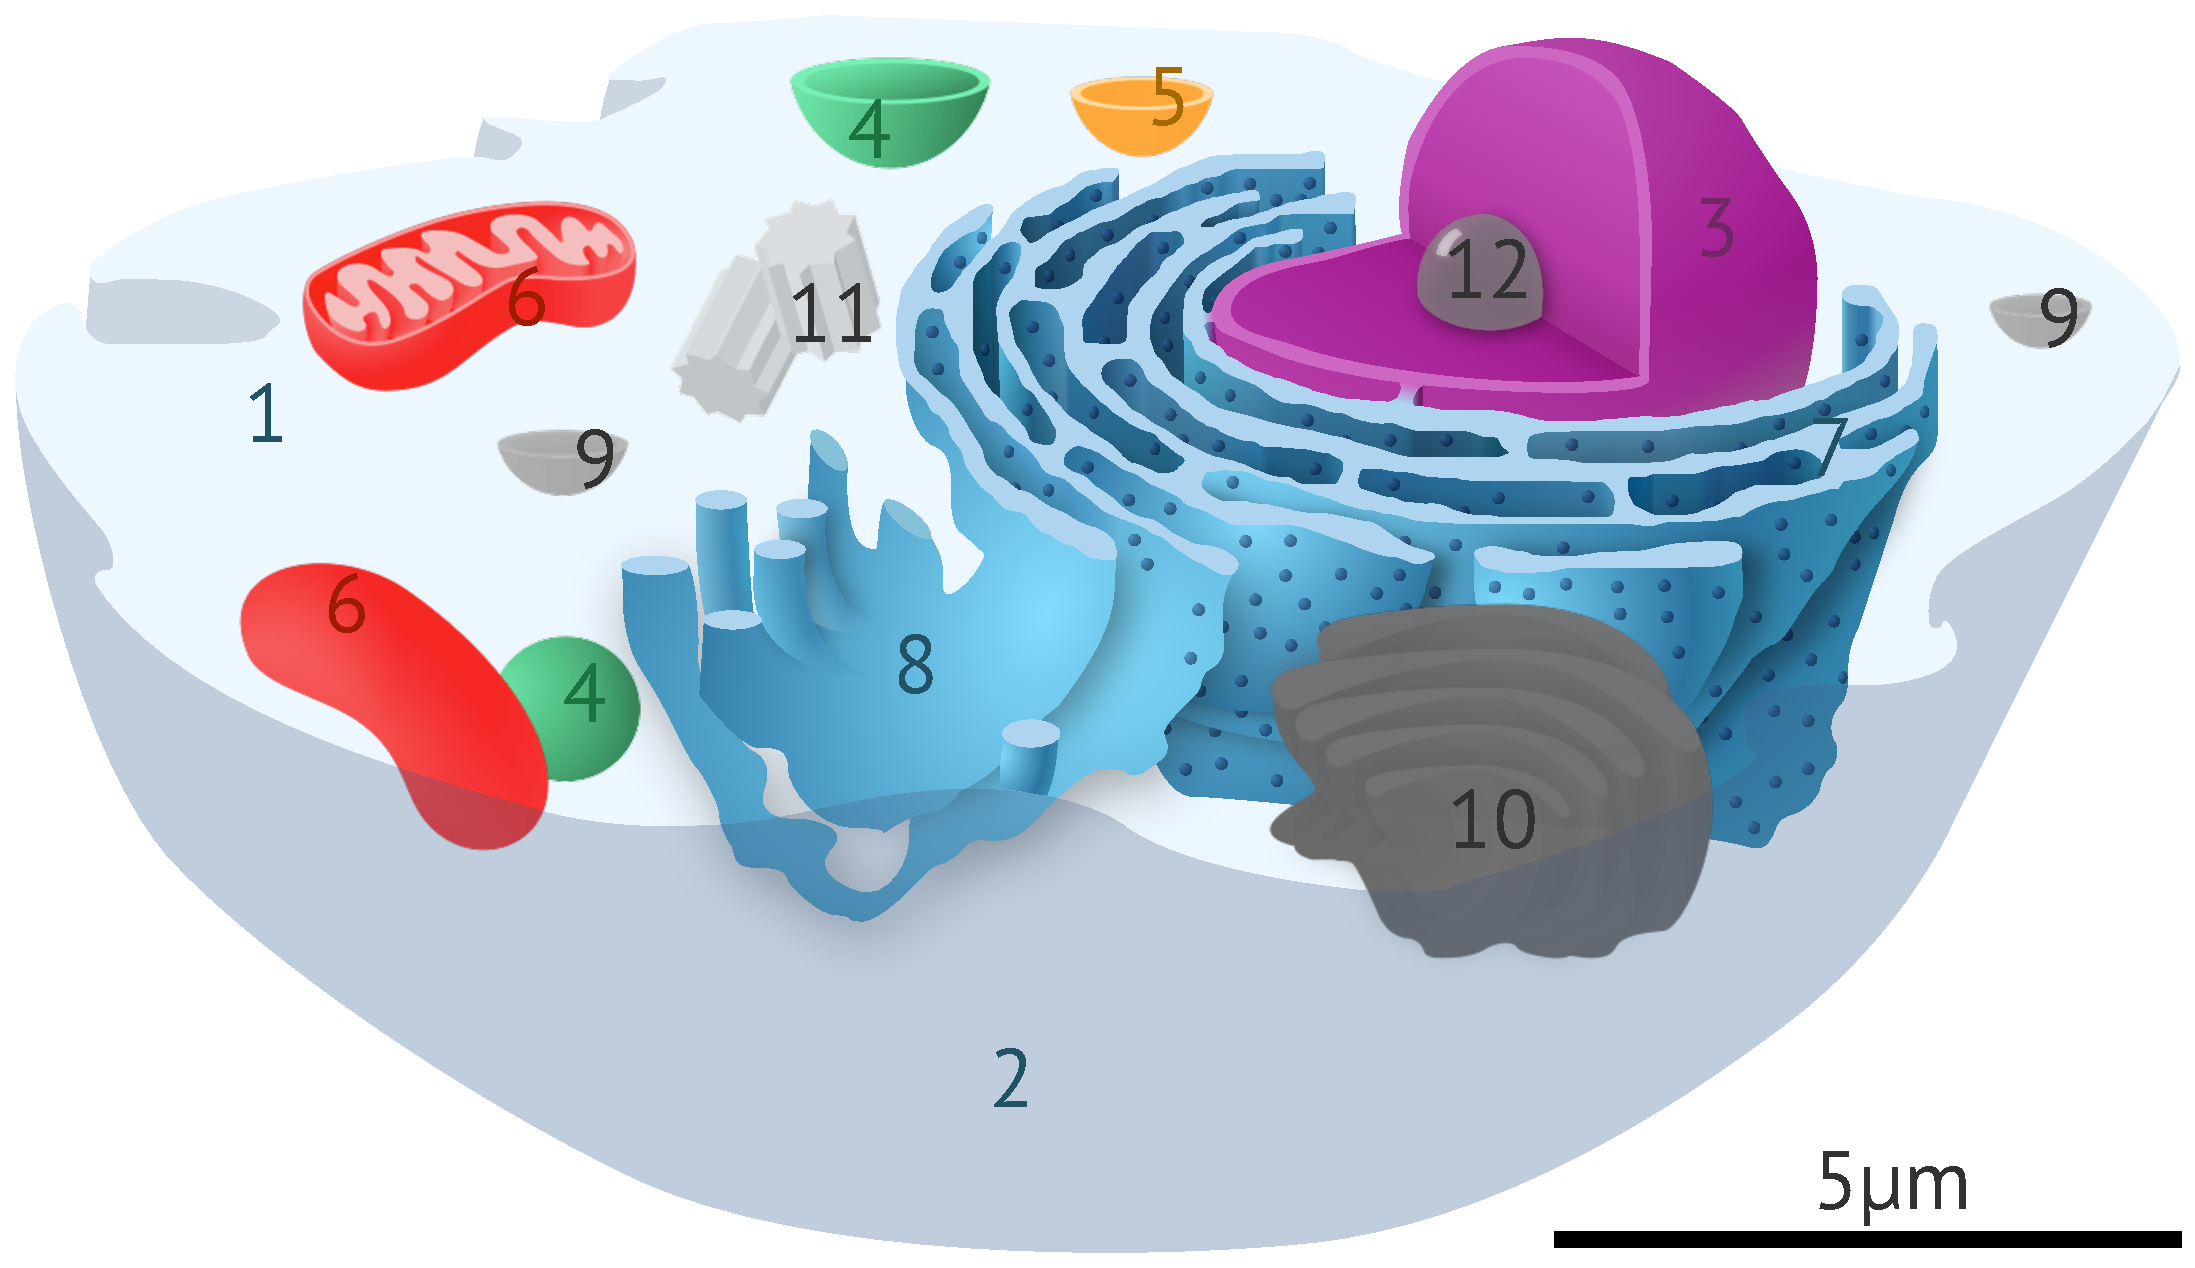
\includegraphics[width=1.0\textwidth]{animal-cell}
\captionsetup{singlelinecheck=off}
\caption[Introduction: Animal cell labelled with organelles relevant to this thesis]{A generic animal cell, adapted from Wikipedia\cite{wikicell}, but with the organelles discussed in this thesis highlighted in colour. Numbered annotations are as follows:\newline
\begin{tabular}{p{0.3\textwidth}p{0.3\textwidth}p{0.3\textwidth}}
\begin{enumerate} 
	\item Cytosol 
	\item Cell membrane 
	\item Nucleus 
	\item Lysosome 
\end{enumerate} &
\begin{enumerate} \setcounter{enumi}{4}
	\item Endosome 
	\item Mitochondria 
	\item ER network 
	\item ER sheets 
\end{enumerate} &
\begin{enumerate} \setcounter{enumi}{8}
	\item Vesicle 
	\item Golgi apparatus 
	\item Centrosome 
	\item Nucleolus
\end{enumerate} \\
\end{tabular}} % end of caption!
\label{fig:animal-cell}
\end{figure}

I have included a diagram of the cell, with the compartments relevant to this thesis highlighted.


\section{Structure and aims of this document}
Since October 2015, I have been working in the Laser Analytics Group building tools and applying them to answer biological questions. 

% some other things. 

Finally, this document provides a memento to myself of my PhD experience. 
I am proud of what I have achieved alongside my collaborators, and have included some of my favourite quotes at the start of each chapter. 
I hope these do not come across as arrogant or self-praising; they simply serve as a reminder to myself that others appreciate my hard work and that the effort has undoubtedly been worth it. 


% Nomenclature command could be useful. 